%!TEX root = ../thesis.tex

\section{Local Deployment}
\label{sec:local_infrastructure}

The local deployments consists of the residential communication gateway and the deployed thermostats with their wireless adapters.
The communication gateway collects the data read from the thermostats and sends it to the remote web server.
The thermostats are programmable and allow us to modify their behavior by flashing custom firmware.
This project uses the work of previous lab projects as a basis to build upon.
The primary focus is to improve the basic functionality of the communication gateway and create an unified but loosely coupled infrastructure by using the RESTful API provided by the server.
See also Figure~\ref{fig:residence_layout} for an overview of the local deployment.

\begin{figure}[h]
	\begin{center}
		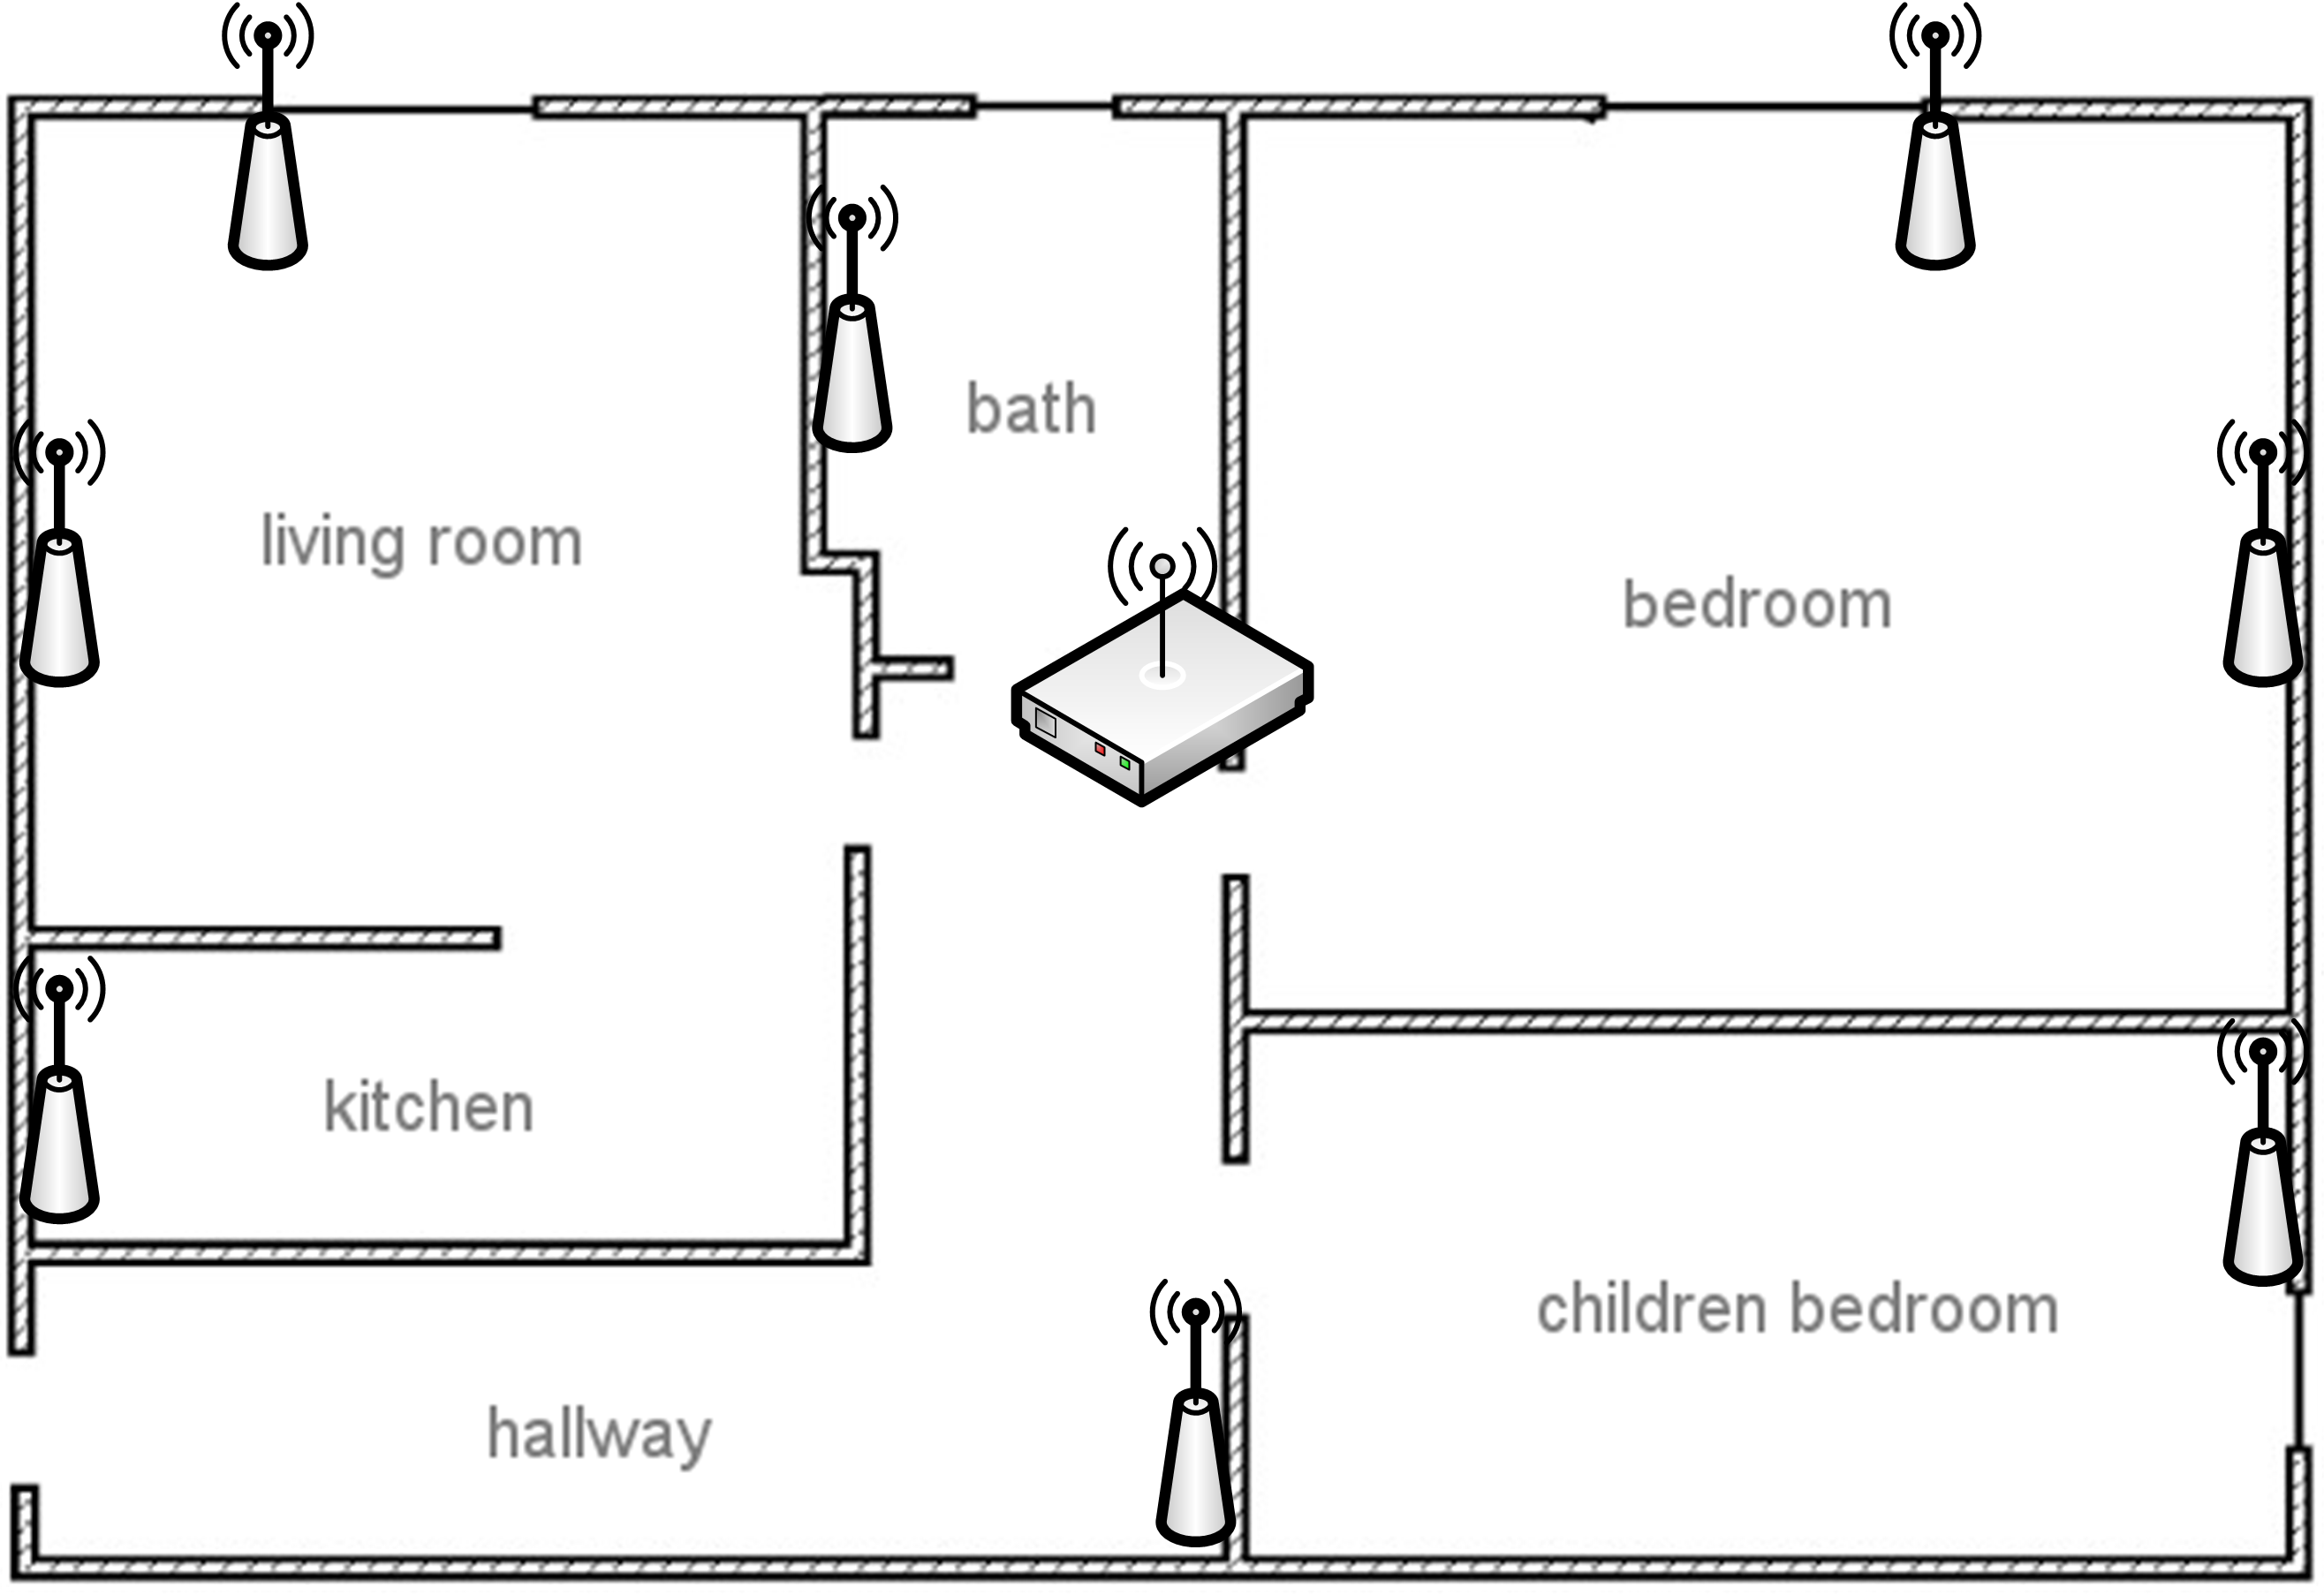
\includegraphics[width=0.7\textwidth]{images/residence_layout_schema.png}
	\end{center}
	\caption{Example of a residence layout depicting a possible deployment. The local communication gateway is installed in the hallway, connected to the internet and has wireless connections to the deployed thermostats represented as antennas. Source of the original image: \url{http://www.haus-topplicht.de/wp-content/uploads/2013/12/planwohnung2.jpg}}
	\label{fig:residence_layout}
\end{figure}

\subsection{Existing Infrastructure}

This project builds upon work previously done by Nico Eigenmann as his master thesis \cite{eigenmann2012opportunisticSensing}.
Part of his work consisted of extending the hardware and software of the digital thermostat HR-20\footnote{\url{http://www.homexpertbyhoneywell.com/en-DE/Products/rondostat/Pages/HR-20.aspx}}, as depicted in Figure~\ref{fig:honeywell_hr20}, to offer wireless access via 6LoWPAN\footnote{Acronym of IPv6 over Low power Wireless Personal Area Network}.
Further a border router translates the 6LoWPAN messages into IPv6 packets and vice versa.
This border router is connected per Universal Serial Bus (USB) port to a computer and communicates via Serial Line Internet Protocol (SLIP).
The computer redirects the received messages into the connected Local Area Network (LAN) and also routes packets addressed to a sensor in the 6LoWPAN network via the border router.

\begin{figure}[h]
%\begin{wrapfigure}{r}{0.45\textwidth}
	\begin{center}
		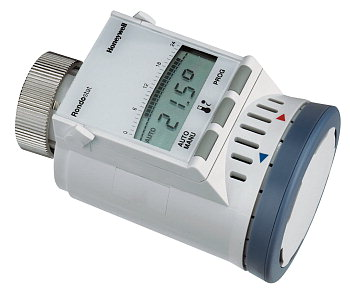
\includegraphics[width=0.4\textwidth]{images/hr20.jpg}
	\end{center}
	\caption{Honeywell Rondostat HR-20 programmable thermostat. Image source: \url{https://piontecsmumble.files.wordpress.com/2013/02/hr20.jpg}}
	\label{fig:honeywell_hr20}
\end{figure}

\subsection{Design Goals}

Several design goals are determined in order to evaluate the system design and implementation.

\begin{itemize}
	\item \emph{Performance} for low computational effort and power consumption on embedded systems.
	\item \emph{Reliability} for a high probability to operate as expected.
	\item \emph{Robustness} to let the system behave reasonably in presence of failures.
	\item \emph{Interoperability} to cooperate with other distributed systems.
\end{itemize}

\subsection{Software Platform and Frameworks}

This sub section lists and describes the software components used in the local deployment.

tunslip6, Python, COAP, aiocoap, requests

\paragraph{Constrained Application Protocol (CoAP)}
Targets small low power devices and components that are heavily restricted in terms of computing power, memory size and power consumption.
"CoAP is designed to easily translate to HTTP for simplified integration with the web, while also meeting specialized requirements such as multicast support, very low overhead, and simplicity."

\paragraph{aiocoap} is a package for Python implementing the CoAP protocol.

\paragraph{tunslip6}
% https://www.iot-lab.info/tutorials/build-tunslip6/
"Tunslip creates a virtual network interface (tun) on the host side and uses SLIP (serial line internet protocol) to encapsulate and pass IP traffic to and from the other side of the serial line. The network element sitting on the other side of the line does a similar job with it’s network interface."


\subsection{Implementation}

The communication gateway collects, caches and processes the data read from the thermostats as also the control commands from the server. The local communication gateway works as a proxy server and enables the local deployment to operate independently from the connection to the remote server. This way the last downloaded heating schedule is kept and operated until the server connection is be reestablished.
%Die grundlegende Einheit jedes Deployments ist die Residence. Eine Residence entspricht genau einem installiertem lokalen System, das die gelesenen Daten der Thermostate sowie Steuerbefehle des Servers sammelt, cached and ausführt. Das lokale Gerät arbeitet als ein lokales Gateway und sorgt dafür, dass der lokale Teil unabhängig von der Verbindung mit dem remote Server funktioniert.
% Temperaturen und andere Meta-Daten von den angebundenen Thermostaten sammelt und cached.

\todo[inline]{Overview picture the used local deployment: thermostat, radio module powerd by USB, Raspbeery with border router}
Honeywell HR-20, Radio Module deRFmega128, USB powered

